\section{Intent Resolution}

We now move onto utilizing elements of planning, from which we deal with
the problem of intent resolution within our CAIS.
Ideally, any action carried out by our humans within the room would be as explicit
as possible. Indeed, when using something like MUIFOLD, this explicitness is handled for
the user under the hood by the app, tying together what note or block they're interacting
with, and what action they're attempting to accomplish with it. However, through voice,
providing the full explicit action may be difficult or 
impossible~\cite{kephart_embodied_2019}. To demonstrate this
behavior in more exact terms, we provide a motivating example. Imagine that within a CAIS, there
are two agents working with the sticky notes domain. Similar to work shown by
Bolt~\cite{bolt_put-that-there:_1980} a user may point to a note and say "Delete that
note". Alternatively, for reference a note by color on the screen, a user may say "Delete the blue
note". In both cases, while our system provides us with a ``\delete'' intent, we are not
provided an exact note we wish to operate on, and the system has to determine it from
context. We now talk through our algorithm for resolving the intent into something that
is actionable by our system.

\begin{figure}
\centering
  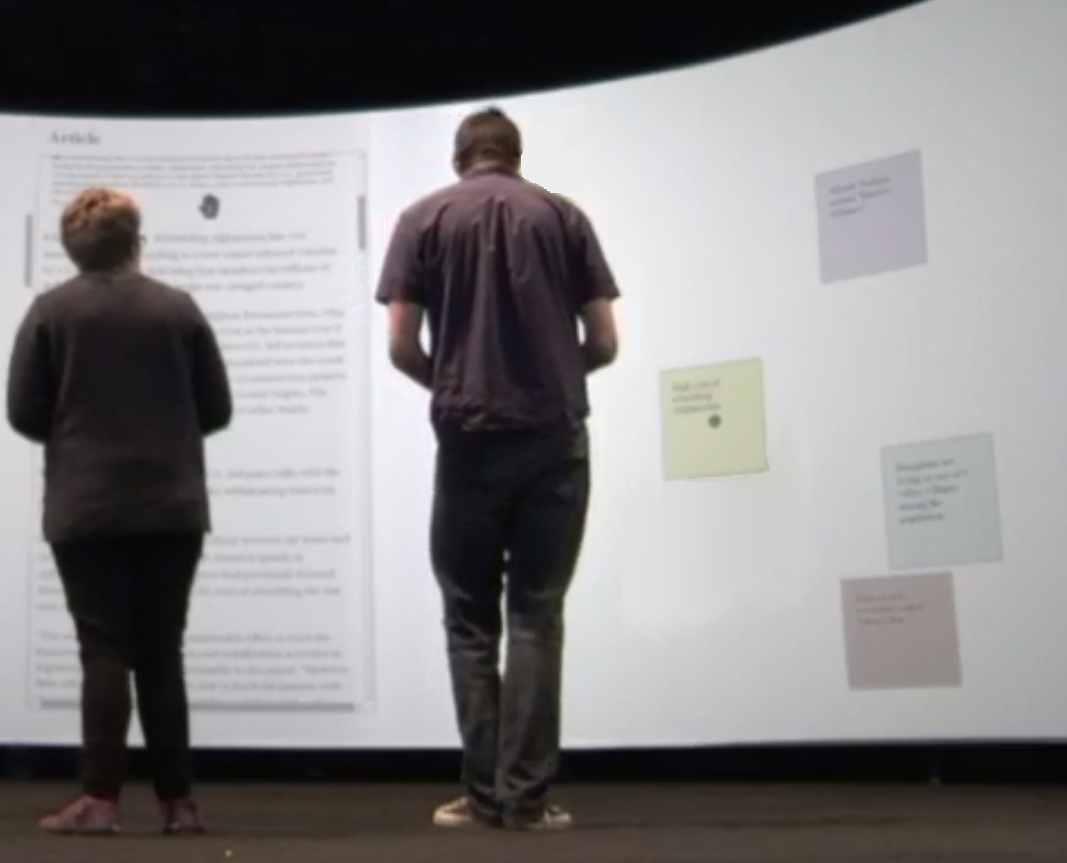
\includegraphics[width=0.7\columnwidth]{chapters/06_planning/figures/intent_sticky_notes.png}
  \caption{Analyst using sticky notes application.}
  \label{fig:intent_sticky_notes}
\end{figure}

We start with grounding our example into a real-world scenario, shown in
Figure~\ref{fig:intent_sticky_notes}. In this scenario, we have two agents once again, \humana\ and
\humanb. There are four notes on the screen, $n1$, $n2$, $n3$, and $n4$ that each have their own color
and location on the screen. Agent \humanb\ is currently pointing at note $n1$ on the screen. We can
axiomatize this set-up as follows:

\begin{center}
\begin{tabular}{ l l l }
    $\holds(\onScreen(n1), 0)$ & 
    $\holds(\position(n1, 50, 50), 0)$ &
    $\holds(\isColor(n1, yellow), 0)$ \\
    $\holds(\onScreen(n2), 0)$ &
    $\holds(\position(n2, 75, 30), 0)$ &
    $\holds(\isColor(n2, purple), 0)$ \\
    $\holds(\onScreen(n3), 0)$ &
    $\holds(\position(n3, 80, 65), 0)$ &
    $\holds(\isColor(n3, blue), 0)$ \\
    $\holds(\onScreen(n4), 0)$ &
    $\holds(\position(n4, 75, 85), 0)$ &
    $\holds(\isColor(n4, red), 0)$ \\
    $\happens(\point(\humanb, n1), 0)$
\end{tabular}
\end{center}

We start first with our example of "Delete that note" as uttered by \humanb. From the conversation-worker,
we receive the \delete\ intent with no further entities. Our orchestrator upon receving the intent then
reaches out to the executor to determine if there are any matching actions to the intent, and receives
the following action, as defined in our STRIPS-style langauge:


\begin{lstlisting}[caption=delete,mathescape=true]
    (define-action delete [(Note ?x)]
        {
            :preconditions [(onScreen ?x)]
            :additions     []
            :deletions     [
                (onScreen ?x)
                $\forall$(y, z) (position ?x y z)
            ]
        }
    )
\end{lstlisting}

From this action, the orchestrator determines that we need a \Note entity to complete the
action, and that we did not receive any such entity from the parsed statement. As such,
the orchestrator then looks to see if it can determine a \Note entity from our context. Here,
it looks through perceived actions of the two agents, scanning in time descending order through
our knowledge base until it finds an action that happened against a note. For our example, it
quickly matches against $\happens(\point(\humanb, n1), 0)$, and given that this action happened
on the same moment as our utterance, then \Note\ $n1$ is deleted. What about had our other agent,
\humana, uttered the statement instead? From our definition of \vicinity and its relation to \perceives
as defined in Chapter~\ref{chap:formalizing}, we know that \humana has perceived the pointing action
by \humanb. Our orchestrator utilizes that to resolve our intent to the same note in this case.
If both agents were pointing at a note, then the system resolves first to actions committed by that
agent over the ones committed by other agents at the same moment. Finally, the orchestrator
only considers actions that have happened in the recent past (e.g. in the last minute), attempting
to capture the length of attention upon which an agent may give to a particular action or event in
the system. If there is no note that fits our criteria, then the orchestrator issues a request
to the user to clarify which note that they mean.

We now move to our other example of "Delete the yellow note". Similar to above, the orchestrator
gets the same action from the executor and cannot resolve it against any entity in the utterance.
Unlike above however, our utterance contains the \Color\ entity, which is a property of notes and so the
orchestrator then knows that it is additionally looking for a yellow note, or as defined in the
\CEC: $\holds(\isColor(?x, yellow), 0)$. Given this property and the precondition from our action,
our orchestrator generates the query "does there exist a note that is on the screen and is
yellow?" which is formalized as following:

\begin{equation*}
    \exists (\Note\ x, 0) (\holds(\onScreen(x), 0) \land \holds(\isColor(x, green), 0))
\end{equation*}

This query is run through \textsf{ShadowProver} as many time as necessary to determine
the candidate set of notes that fit our needs. To accomplish this, for each candidate
returned, we then re-run our query appending a $(x \neq n)$ where $n$ is our discovered
note candidate in the previous step. We keep on appending discovered candidates until the orchestrator
hit a point where \textsf{ShadowProver} can no longer return any matching note. In the case
that the system receives only one note that fits the above query, that note is then removed.
If there are two or more notes, we then utilize a similar algorithm as above, where the
orchestrator scans for actions that relate to any of our candidate notes. If the system
finds any such action within a similar time frame (such as we have in our example), that note
is then used over any other candidate. Similar to above, if there is no way to determine
which note that the user referred to, the system then asks the user to clarify which
note they were referring to.

\begin{figure}
\centering
  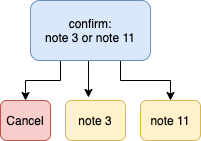
\includegraphics[width=0.3\columnwidth]{chapters/06_planning/figures/intent_resolution_fragment.png}
  \caption{Conditional plan fragment to ask clarification from user.}
  \label{fig:intent_resolution_fragment}
\end{figure}

For cases in which the orchestrator goes back to the user, our system utilizes a similar concept
as employed by Botea et al.~\cite{botea_generating_2019}, where the question to the user
is generated by the orchestrator based on possible candidates and timing, and sets itself up
to expect specific answer types here. For example, let's assume we had two notes that matched
our deletion query. The orchestrator then asks the user for clarification between the two notes
as shown in Figure~\ref{fig:intent_resolution_fragment}, expecting that the response (ignoring
any detected intent) contains one of the notes, or is totally unrelated, thus cancelling the
information request, and continuing as normal. 
